\chapter{Phân tích các hệ điều khiển có trễ sử dụng phương pháp hàm Lambert W}
\setlength{\parindent}{6.5ex}

\indent Trong chương này ta trình bày tổng quan về phương pháp tiếp cận sử dụng hàm Lambert W để nghiên cứu các hệ điều khiển có trễ. 
Cách tiếp cận này đã được xây dựng và phát triển để phân tích và điều khiển các hệ có trễ tuyến tính, hệ số hằng với một trễ hằng số biết trước (đơn trễ). 
Biểu diễn nghiệm trong miền thời gian được xây dựng dưới dạng chuỗi vô hạn, với đặc tính là chuỗi chặt cụt sẽ cho ta phần trội (dominant part) của nghiệm 
của hệ điều khiển ban đầu, mà nó chứa các giá trị riêng nằm ngoài cùng bên phải. 
Trước hết công thức nghiệm được xây dựng cho các hệ bậc nhất (hệ vô hướng), và sau đó được phát triển cho hệ bậc cao bất kỳ bằng việc sử dụng cách tiếp cận hàm Lambert. Các công thức biểu diễn nghiệm được sử dụng để nghiên cứu những tính chất cơ sở của lý thuyết điều khiển cho các hệ điều khiển có trễ, ví dụ như tính điều khiển được, tính quan sát được. 
% Ngoài ra, thông qua việc thiết kế giá trị riêng, quy tắc phản hồi và quan sát trạng thái cũng sẽ được xây dựng để đạt được kết quả mong muốn. Tất cả những tính chất này đều có thể đạt được bằng cách sử dụng cách tiếp cận thông qua hàm Lambert W. Bên cạnh đó, thông qua các ví dụ mô phỏng số, ta sẽ đi tìm hiểu gói công cụ mã nguồn mở \textbf{LambertWDDE} trong ngôn ngữ tính toán khoa học \textbf{MATLAB}.

\section{Giới thiệu chung}

Hệ điều khiển có trễ nảy sinh trong rất nhiều bài toán trong tự nhiên và kỹ thuật, chẳng hạn như trong các quá trình với trễ vận chuyển, các bài toán dòng giao thông, các hệ sinh học, viễn thông và còn rất nhiều vấn đề khác. Có rất nhiều tài liệu về các hệ có trễ, bao gồm nhiều cuốn sách và bài tổng quan, xem \cite{BelC63,Gu06,Hal63,Kol99,Ric03,Sip11,Ste89} và các tài liệu trong đó. Chương này tập trung vào một cách tiếp cận đặc biệt và được phát triển gần đây, dựa trên cách tiếp cận sử dụng hàm Lambert W, \cite{Cor96}, để phân tích và điều khiển các hệ điều khiển tuyến tính, hệ số hằng với đơn trễ, \cite{Yi10}.

Xét một hệ điều khiển không trễ dạng \eqref{1} với công thức nghiệm tường minh \eqref{sol}. Bởi vì hệ phương trình vi phân thường trong \eqref{1} có phổ hữu hạn, tính ổn định của hệ có thể được xác định bằng cách kiểm tra các vị trí của một số hữu hạn các giá trị riêng trong mặt phẳng phức. Bên cạnh đó, công thức nghiệm của hệ này cũng được sử dụng để xây dựng các ma trận điều khiển Grammian và ma trận quan sát Grammian. Từ đó, tính điều khiển  và tính quan sát sẽ được kiểm tra bằng cách điều kiện hạng của ma trận điều khiển Grammian và ma trận quan sát Grammian tương ứng, như đã được trình bày trong Mục \eqref{sec1.2}. 
%
Thêm vào đó, nếu hệ đã cho là điều khiển được thì một bộ (thiết bị) điều khiển (controller) đóng kín có thể được thiết kế bằng nhiều phương pháp, bao gồm cả điều khiển phản hồi và phương pháp thiết kế giá trị riêng (eigenvalue assignment). Tương tự, nếu một hệ có thể quan sát được, sau đó, một bộ quan sát (observer) hay bộ ước lượng trạng thái (state estimator) cũng có thể được thiết kế bằng cách sử dụng phương pháp thiết kế giá trị riêng. 
Đối với các hệ phương trình trạng thái dạng \eqref{1}, bởi vì ta có công thức nghiệm tường minh nên các bước nghiên cứu đề cập ở trên có thể thực hiện được một cách đơn giản.

Mặc dù vậy, đối với các phương trình vi phân có trễ thì công thức nghiệm tường minh là chưa có, và do đó các bước nghiên cứu ở trên sẽ khó có thể thực hiện hơn nhiều. Để tìm nghiệm (nghiệm giải tích hoặc nghiệm số), thông thường phương pháp các bước (method of steps) được thực hiện nhằm tìm ra công thức nghiệm hay tính toán nghiệm xấp xỉ một cách tuần tự trên các đoạn $[0,h]$, $[h,2h]$, $[2h,3h]$,... 
Bên cạnh đó, do sự tồn tại của trễ $h>0$ mà phổ của hệ là một tập có vô hạn phần tử. Để vượt qua những khó khăn này, gần đây phương pháp hàm Lambert W đã được đề xuất, chứng minh và phát triển nhằm nghiên cứu các hệ điều khiển có trễ theo cách tương tự với các phương trình trạng thái dạng \eqref{1} (\cite{AslU03,YiEig10}). Đặc trưng của phương pháp này là sử dụng các nhánh của hàm Lambert W để biểu diễn nghiệm dưới dạng một chuỗi vô hạn với biến số là các giá trị riêng của hệ điều khiển có trễ đang xét. Trên cơ sở đó, ta sẽ tìm cách cắt gọn để thu được một chuỗi chặt cụt hữu hạn sao cho nó chứa tất cả các giá trị riêng trội (các giá trị riêng có vai trò quyết định dáng điệu của nghiệm). 

Trong tự nhiên và kỹ thuật có rất nhiều hệ điều khiển mà trong đó xuất hiện độ trễ thời gian, ví dụ như các hệ sinh học, mô hình kinh tế, chuỗi cung ứng, lưu lượng giao thông, viễn thông, hệ điều khiển mạng lưới, hệ điều khiển ô tô, xem \cite{Sip11}. 
Do đó, việc mở rộng các công cụ phân tích và điều khiển đã biết đối với phương trình dạng \eqref{1} (ODEs) cho các hệ điều khiển có trễ (DDEs) là rất quan trọng. \
%
Chương này nhằm cung cấp một cái nhìn tổng quan và súc tích về phương pháp hàm Lambert W nhằm phân tích và điều khiển các hệ đơn trễ với trễ hằng số thông qua các ví dụ số đơn giản. 
Để thực hiện các thử nghiệm số, ta sẽ sử dụng gói công cụ nguồn mở LambertWDDE, có sẵn để tải xuống từ trang web \cite{Dua10}. 
Các ví dụ bổ sung có thể được tìm thấy tại cùng trang web \cite{Dua10}. Nhiều ứng dụng khác của phương pháp này có thể được tìm thấy trong các tài liệu tham khảo được trích dẫn (ví dụ \cite{Du12,Sip11,Yi07,Yi08,YiOc08,Yi10,Yi13})  


\section{Ứng dụng của hàm Lambert W trong lý thuyết phương trình vi phân có trễ}

\subsection{Trường hợp vô hướng}
\noindent Trước hết chúng ta xét hệ điều khiển trong đó cả biến điều khiển $u(t)$ và biến trạng thái $x(t)$ đều là vô hướng
%
\begin{equation}\label{3}
\dot{x}(t)=ax(t)+a_dx(t-h)+bu(t),
\end{equation} 
%
trong đó $a$, $b$, $a_d$ là các hằng số đã biết và $h$ là trễ hằng số. Điều kiện ban đầu $x(0)=x_0$ và $x(t)=g(t)$ với mọi $-h\leq t<0$ phải được cho trước. Hàm Lambert W được áp dụng để giải phương trình đặc trưng được viết lại dưới dạng
\begin{equation}\label{4}
(s-a)e^{sh}=a_d.
\end{equation} 
Nhân cả hai vế của phương trình \eqref{4} với $he^{-ah}$ ta nhận được
\begin{equation}\label{5}
h(s-a)e^{h(s-a)}=a_dhe^{-ah}.
\end{equation}
Dựa trên định nghĩa của hàm Lambert W trong biểu thức \eqref{5} ta có
\begin{equation}\label{6}
W(a_dhe^{-ah})e^{W(a_dhe^{-ah})}=a_dhe^{-ah}.
\end{equation} 
So sánh các phương trình \eqref{5} và \eqref{6} ta có
\begin{equation}\label{7}
h(s-a)=W(a_dhe^{-ah}).
\end{equation} 
Do đó, nghiệm của phương trình đặc trưng trong phương trình \eqref{4} có thể được viết theo hàm Lambert W như
\begin{equation}\label{8}
s=\dfrac{1}{h}W(a_dhe^{-ah})+a.
\end{equation} 
Phổ của phương trình DDE vô hướng \eqref{3} thu được bằng cách sử dụng vô hạn nhánh của hàm Lambert W, và được trình bày tường minh theo các tham số $a, a_d$ và $h$ của hệ. Các nghiệm của phương trình đặc trưng \eqref{4}, cho $k=0,\pm 1,\pm 2,\cdot, \pm\infty$ là
\begin{equation}\label{9}
s_k=\dfrac{1}{h}W_k(a_dhe^{-ah})+a.
\end{equation}
Hơn nữa, đối với phương trình \eqref{3} tích chất ổn định được xác định bởi giá trị riêng bên phải (nửa phổ phải) của mặt phẳng phức (tức là, $k = 0$). Do đó, để đảm bảo sự ổn định, không cần thiết phải kiểm tra các giá trị riêng khác trong phổ vô hạn.

\begin{vd}\label{vidu1}
	Cho $a=-1, a_d=0.5,$ và $h=1$ các nghiệm đặc trưng thu được bằng phương trình \eqref{9} và hàm \emph{lambertw} trong MATLAB, và được vẽ trong Hình \ref{refhinh1}.
	\begin{figure}[h]
		\centering
		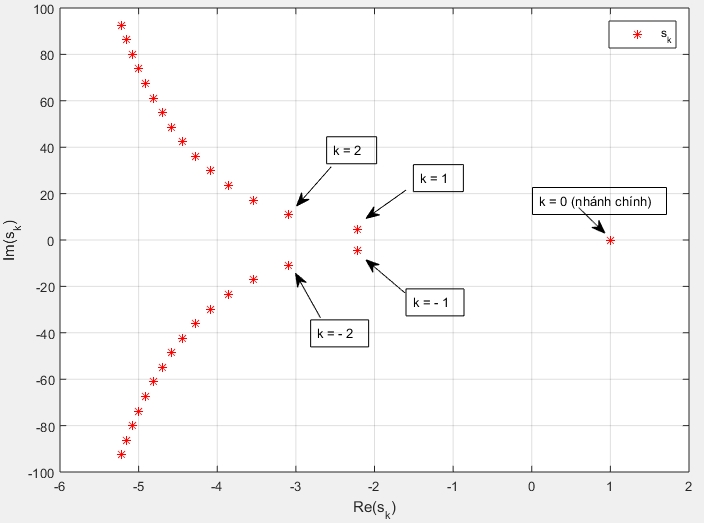
\includegraphics[width=0.9\linewidth]{hinh/hinh1}
		\caption{Giá trị riêng của phương trình \eqref{3} khi $a=-1, a_d=0.5,$ và $h=1$. Giá trị riêng bên phải là tương ứng với nhánh chính $k=0$, các cặp tiếp theo lần lượt tương ứng với $k=\pm 1, \ \pm 2, \dots, \pm 15$.}
		\label{refhinh1}
	\end{figure}
\end{vd}

Trong \cite{YiEig10} nghiệm tổng quát của phương trình \eqref{3} được biểu diễn dưới dạng một chuỗi vô hạn dựa trên các giá trị riêng trong công thức \eqref{9} như sau
\begin{equation}\label{10}
x(t)=\sum\limits^{+\infty}_{k=-\infty}e^{s_kt}C^I_k+\int^t_0\sum\limits^{+\infty}_{k=-\infty}e^{s_k(t-\eta)}C^N_kbu(\eta)d\eta \ ,
\end{equation} 
trong đó
\begin{equation}\label{11}
C^I_k=\dfrac{x_0+a_de^{-s_kh}\int^h_0e^{-s_kt}g(t-h)dt}{1+a_dhe^{-s_kh}} \quad ,
\end{equation} 
và
\begin{equation}\label{12}
C^N_k=\dfrac{1}{1+a_dhe^{-s_kh}} \quad .
\end{equation} 
Lưu ý rằng các hệ số $C^I_k$ được xác định từ hàm $g(t)$ và trạng thái ban đầu $x_0$, và các hệ số $C^N_k$ chỉ được xác định theo các tham số hệ $a, a_d$ và $h$. Do đó, nghiệm tổng quát của phương trình \eqref{10} có thể được xem là tổng của một nghiệm của hệ thuần nhất (mà chúng ta sẽ gọi là \emph{nghiệm tự do (free solution)}) và một nghiệm riêng của hệ không thuần nhất (mà chúng ta sẽ gọi là \emph{nghiệm chịu lực tác động (forced solution)}). 

Các điều kiện để hội tụ của các nghiệm dạng chuỗi như vậy được thảo luận bởi Bellman và Cooke trong \cite{BelC63}. Ví dụ, nếu tất cả mọi giá trị riêng $s_k$ đều có phần thực âm và tồn tại một chặn dưới dương cho khoảng cách giữa các giá trị riêng
thì chuối vô hạn nói trên sẽ hội tụ. 
%
Một khía cạnh khác rất quan trọng của biểu diễn dạng chuỗi này của nghiệm $x(t)$ đó là việc chặt cụt chuỗi, ví dụ $k=0,\pm 1,\pm 2,...,\pm n$, sẽ dẫn đến một xấp xỉ cho nghiệm $x(t)$ dựa trên tối đa $(2n + 1)$ giá trị riêng ngoài cùng bên phải (còn được gọi là các giá trị riêng trội). Hệ quả là ta có thể xây dựng một biểu diễn xấp xỉ hữu hạn chiều cho hệ \eqref{3} mà vẫn giữ nguyên được các tính chất động lực của hệ.   

\begin{vd}\label{vidu2} (Xấp xỉ phản hồi trong trường hợp vô hướng)
	Cho $a=-1, a_d=0.5$, $b=1$ và $h=1$ ta có thể tìm được các giá trị của $s_k$ thông qua biểu thức \eqref{9} và hàm Lambert W như trong Ví dụ \ref{vidu1} và các giá trị của $C^I_k$ và $C^N_k$ sử dụng các phương trình \eqref{11} - \eqref{12}, trong đó $x_0=1$ và $g(t)=1$ với $-h\leq t<0$. Các giá trị riêng $s_k$ và các hệ số này được trình bày trong Bảng \eqref{bang1}. Hình \ref{refhinh2} thể hiện phản hồi cho trường hợp $u(t)=\sin(t)$ và so sánh giữa phương pháp dựa trên hàm Lambert W (sử dụng 7 thành phần trong Bảng \eqref{bang1}) và nghiệm số (sử dụng hàm dde23 trong MATLAB). 
	%
	\begin{figure}[ht]
		\begin{center}
			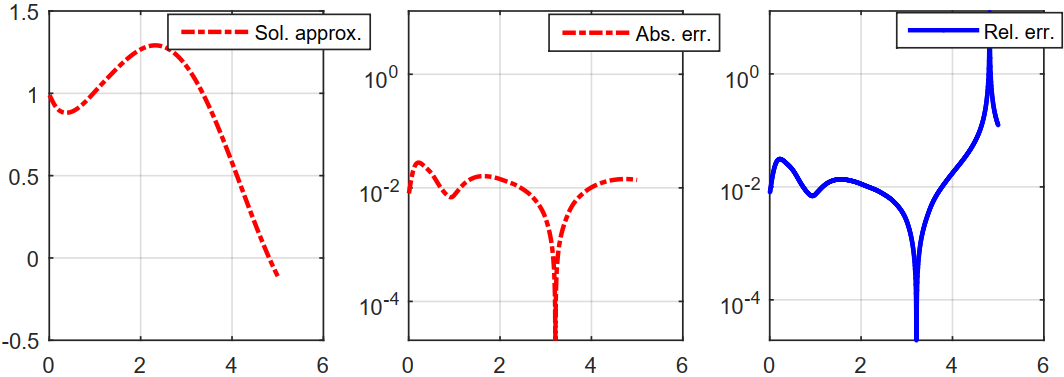
\includegraphics[scale=0.55]{hinh/hinh2}
		\end{center}
		\caption{Phản hồi cho trường hợp $u(t)=\sin(t)$, với $x_0=1$ và $g(t)=1$ cho $-h\leq t<0$, và so sánh giữa công thức chặt cụt nghiệm giữ 7 thành phần đầu tiên dựa trên phương pháp hàm Lambert (xem Bảng \eqref{bang1}) và phương pháp số (hàm dde23 trong MATLAB). Các hệ số là $a=-1, a_d=0.5$, và $h=1$.}
		\label{refhinh2}
	\end{figure}
	%
	
	\begin{table}[ht]
		\centering	
		\begin{tabular}{llll}
			\hline \\[-.35cm]
			k & $s_k$ & $C^I_k$ & $C^N_k$ \\ 
			\hline 
			0 & $-0.3149$ & 1.0713 & 0.5934 \\ 
			
			$\pm1$ & $-2.2211\pm 4.4442$ i & $-1.9829 \pm  0.4711$ i & $-0.0112\pm 0.2245$ i \\ 
			
			$\pm2$ & $- 3.0915\pm 10.8044$ i & $-2.0109 \pm  0.1863$ i & $- 0.0093\pm 0.0916$ i \\ 
			
			$\pm3$ & $- 3.5450 \pm 17.1313$ i & $-2.0073 \pm  0.1168$ i & $- 0.0052 \pm  0.0579$ i \\ 
			
			$\pm4$ & $-3.8550 \pm  23.4407$ i & $-2.0050 \pm  0.0852$ i & $-0.0034 \pm  0.0424$ i  \\
			
			$\pm5$ & $ -4.0911 \pm  29.7416$ i & $-2.0036 \pm  0.0671$ i & $-0.0024 \pm  0.0335$ i \\
			
			\hline 
		\end{tabular}
		\caption{Các giá trị riêng và hệ số trong Ví dụ \ref{vidu2}}
		\label{bang1} 
	\end{table}%
\end{vd} 

\subsection{Trường hợp hệ phương trình}
\noindent Phép xấp xỉ được trình bày trong phần trước đã được khái quát hóa trong \cite{Yi10} cho hệ điều khiển có trễ có dạng sau
%
\begin{align}\label{13}
\dot{x}(t) & =Ax(t)+A_dx(t-h)+Bu(t), \\
y(t)&=Cx(t)+Du(t), \notag 
\end{align}
%
trong đó $x(t)$ là vectơ trạng thái, $u(t)$ là biến điều khiển, $y(t)$ là vectơ đầu ra, $A, A_d, B, C$ và $D$ là các ma trận hệ số và $h$ là độ trễ vô hướng đã biết. Điều kiện ban đầu $x(t=0)=x_0$ và $x(t)=g(t)$ với $-h\leq t <0$ phải được cho trước. Công thức nghiệm cho hệ \eqref{3} có dạng:
%
\begin{equation}\label{14}
x(t) = \sum\limits^\infty_{k=-\infty}e^{S_kt}C^I_k+\int^t_0\sum\limits^\infty_{k=-\infty}e^{S_k(t-\eta)}C^N_kBu(\eta)d\eta,
\end{equation} 
trong đó
\begin{equation}\label{15}
S_k=\dfrac{1}{h}W_k(A_dhQ_k)+A,
\end{equation} 
và $Q_k$ được lấy từ nghiệm số (như bằng cách sử dụng hàm $fsolve$ trong MATLAB) của phương trình
%
\begin{equation}\label{16}
W_k(A_dhQ_k)e^{W_k(A_dhQ_k)+Ah}=A_dh.
\end{equation} 
%
Ở đây các hàm ma trận Lambert $W_k$ được định nghĩa như trong Mục \ref{sec1.1}. 
Các đại lượng $Q_k, W_k, S_k, C^I_k$ và $C^N_k$ trong các phương trình \eqref{14} - \eqref{16} đều có thể tính được bằng các lệnh trong gói công cụ LambertWDDE theo các điều kiện đã cho $h, A, A_d, g(t), x_0, B$ và $u(t)$. Các hàm chính của gói công cụ LambertWDDE được tóm tắt trong Bảng \ref{bang2}. 

\begin{table}[ht]
	\centering	
	\begin{tabular}{ll}
		\hline 
		Tên & Mô tả \\ 
		\hline 
		$lambertw\_ matrix$ & Tính hàm ma trận LambertW \\ 
		
		$find\_ S_k$ & Tìm $\mathcal{S}_k$ và $\mathcal{Q}_k$ cho một nhánh cụ thể \\ 
		
		$find\_ CI$ & Tính $\mathcal{C}_I$ cho một nhánh cụ thể trong điều kiện ban đầu \\ 
		
		$find\_ CN$ & Tính $\mathcal{C}_N$ cho một nhánh cụ thể \\ 
		
		$pwcont\_ test$ & Thử tính điều khiển được cho hệ có trễ \\ 
		
		$pwobs\_test$ & Thử tính quan sát được cho hệ có trễ \\ 
		
		$cont\_gramian\_dde$ & Ma trận điều khiển Gramian của hệ có trễ \\ 
		
		$obser\_gramian\_dde$ & Ma trận quan sát Gramian của hệ  có trễ \\ 
		
		$place\_dde$ & Phân bổ các giá trị riêng trội của hệ có trễ \\ 
		
		$stabilityradius\_dde$ & Tính bán kính ổn định cho hệ có trễ \\ 
		
		%$examples$ & Liệt kê các ví dụ để sử dụng gói công cụ này, \\
		%& mỗi ô là một ví dụ ngắn và có thể được đánh giá riêng \\ 
		\hline
	\end{tabular}
	\caption{Các hàm chính của gói công cụ LambertWDDE}
	\label{bang2}  
\end{table}


Để có được $S_k$ cho một trường hợp $k$ cụ thể người ta cần giải phương trình \eqref{16} để tìm $Q_k$ trước, sau đó thay thế kết quả vào biểu thức \eqref{15} để lấy được $S_k$. Các bước này được thực hiện trong hàm $find\_Sk$. Lưu ý rằng, hàm ma trận Lambert W, Wk trong biểu thức \eqref{15} và \eqref{16} được tính toán bằng hàm $lambertw\_matrix$, dựa trên phép biến đổi dạng Jordan. Để hiểu rõ hơn toàn bộ quá trình, chúng ta đi tìm hiểu một ví dụ ở đây. 

\begin{vd}\label{vidu2.3} 
	Cho
	\begin{equation*} 
	A= \begin{bmatrix}
	-1&-3 \\
	2&-5
	\end{bmatrix}, \
	A_d=\begin{bmatrix}
	1.66&-0.697\\
	0.93&-0.33
	\end{bmatrix}, \
	% Bu = \m{\cos(t) \\ \sin(t) }, \
	h=1 \ . 
	\end{equation*}
	Để tìm các ma trận $S_k$ chúng ta sẽ sử dụng hàm $find\_Sk$ trong gói công cụ LambertWDDE.
	Đối với nhánh chính, $k = 0$, ta có được:
	\begin{equation*}
	S_0=\begin{bmatrix}
	0.3055&-1.4150\\
	2.1317&-3.3015
	\end{bmatrix}.
	\end{equation*}
	Các giá trị riêng của $S_0$ là $-1.0119$ và $-1.9841$. Tiếp theo, sử dụng $find\_CI$ và $find\_CN$, ta có thể nhận được các hệ số cho nghiệm dạng chuỗi của phương trình \eqref{14}. Ví dụ, nếu ta chọn $u(t)=0,g(t)=0$, và ta có một bước nhảy tại $t=0$ đến $x_0= \m{1 & 1}^T$, ta có thể nhận được (sử dụng $find\_CI$) hệ số cho phản hồi tự do cho $k = 0$ là:
	\begin{equation*}
	C^I_0=\begin{bmatrix}
	0.2635\\
	0.4290
	\end{bmatrix}.
	\end{equation*}
	Do đó, phép xấp xỉ sử dụng một nhánh $k = 0$ cho phản hồi tự do là:
	\begin{equation*}
	x(t)=\begin{bmatrix}
	x_1(t)\\
	x_2(t)
	\end{bmatrix}
	= exp \left(
	\begin{bmatrix}
	0.3055&-1.4150\\
	2.1317&-3.3015
	\end{bmatrix} t
	\right)
	\ 
	\begin{bmatrix}
	0.2635\\
	0.4290
	\end{bmatrix}.
	\end{equation*}
	%
	Ở đây ta sử dụng ký hiệu $\emph{exp}$ để chỉ hàm mũ cho cả trường hợp vô hướng lẫn ma trận. Lưu ý rằng trong MATLAB, hàm mũ của ma trận là hàm \emph{expm}, chứ không phải hàm vô hướng \emph{exp}. Để cải thiện phép xấp xỉ, quy trình này có thể được lặp lại cho các nhánh bổ sung thứ $k$, sau đó sự xấp xỉ dạng chuỗi của nghiệm có thể thu đươc thông qua phương trình \eqref{14} (xem Hình \ref{refhinh3}). Ví dụ, các nhánh $k=\pm 1$ cho ta các ma trận $S_k$ liên hợp phức bổ sung:
	\begin{equation*}
	S_{-1,+1}=\begin{bmatrix}
	-0.3499\pm 4.980i&-1.6253\pm 0.1459i\\
	2.4174\pm 0.1308i&-5.1048\pm 4.5592i
	\end{bmatrix},
	\end{equation*}
	với các hệ số liên hợp phức cho phản hồi tự do với $k = \pm 1$ là:
	\begin{equation*}
	C^I_{-1,+1}=
	\begin{bmatrix}
	0.0909\pm 0.1457i\\
	0.0435\pm 0.1938i
	\end{bmatrix}.
	\end{equation*}
\end{vd}

\begin{figure}
	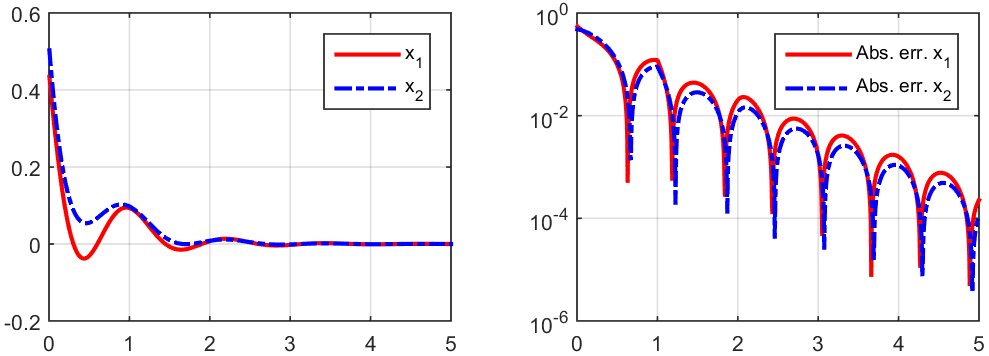
\includegraphics[scale=0.55]{hinh/hinh3_new.png}
	\caption{Phản hồi gần đúng (3 thành phần) và sai số tuyệt đối cho hệ trong Ví dụ \ref{vidu2.3}
	so với nghiệm sử dụng hàm dựng sẵn dde23 trong MATLAB}
	\label{refhinh3}
\end{figure}

%\begin{nx}
%Chú ý rằng trong Ví dụ \ref{vidu2.3} thì hệ có bước nhảy tại thời điểm $t=0$. Vì vậy sai số tuyệt đối/tương đối tại thời điểm $t=0$ còn lớn. Mặc dù vậy sai số sẽ giảm dần theo thời gian.
%\end{nx}

\section{Tính ổn định của hệ}
%
Đối với các hệ thống có trễ dạng \eqref{13} thì tập phổ
%
\begin{equation}\label{spectrum}
\sigma(I,A,A_d) := \{\lb \in \mathbb{C} \ | \ \det(\lb I - A - e^{-\lb h}A_d ) = 0\}
\end{equation}
%
là vô hạn (các giá trị $\lb$ thuộc phổ được gọi là các giá trị riêng của hệ). Chính vì vậy không thể tính được chính xác toàn bộ tập phổ này. Tuy nhiên theo \cite{Hal63} ta biết rằng với mọi số thực $\a$ luôn chỉ có một số hữu hạn các giá trị riêng nằm ở nửa mặt phẳng phải 
$\C^+_{\a}:= \{ \a \in \C \ | \ \Re{\lb}\geq \a \}$.
Chú ý rằng với $\a=0$ thì các giá trị riêng nằm trong $\C^+_{0}$ xác định sự ổn định của hệ thống. Việc tính toán tất cả các giá trị riêng nằm trong $\C^+_{\a}$ với $\a\in \R$ bất kỳ đã được nghiên cứu và thực hiện trong \cite{Eng01}. \\

Điều hết sức thú vị ở đây là đối với trường hợp hệ vô hướng
dạng \eqref{3} thì nhánh chính ($k = 0$) sẽ quyết định tính ổn định của hệ. Điều này đã được Shinozaki và Mori chứng minh trong \cite{Shi06} bằng cách sử dụng tính đơn điệu của phần thực của hàm Lambert W theo chỉ số $k$ của các nhánh (xem Hình \ref{fig1}). \
Thêm vào đó, chứng minh trong \cite{Shi06} có thể được mở rộng cho các hệ có trễ dạng \eqref{13} trong đó $A$ và $A_d$ thỏa mãn điều kiện \emph{tam giác hóa được đồng thời (simultaneously triangularizable)} như trong định nghĩa dưới đây. 
%
\begin{dng}(\cite{RadR00})
Hai ma trận vuông $A$ và $A_d$ được gọi là \emph{tam giác hóa được đồng thời} 
nếu tồn tại một ma trận khả nghịch $T$ sao cho $TAT^{-1}$ và $TA_dT^{-1}$ cùng có dạng tam giác trên.
\end{dng}
%
Chú ý rằng nếu $A$ và $A_d$ là hai ma trận giao hoán thì chúng sẽ là tam giác hóa được đồng thời, xem \cite[Chương 2]{RadR00}.\\
%
\indent Đối với trường hợp tổng quát thì nhánh chính sẽ không còn chứa giá trị riêng với phần thực lớn nhất của phổ, và do đó nhánh chính sẽ không còn vai trò quyết định đến tính ổn định của hệ nữa. 
%
Mặc dù vậy, thông qua quan sát trong nhiều ví dụ thực tế, trong \cite{Yi10} các tác giả đã đưa ra phỏng đoán sau.

\begin{mde}\label{conj}
Xét hệ \eqref{13}. \\
a) Giả sử rằng $0$ không phải là giá trị riêng bội của 
ma trận hệ số $A_d$. Khi đó các giá trị riêng nằm trên nhánh chính $k=0$ sẽ có phần thực lớn nhất. \\
b) Nếu $0$ là giá trị riêng bội của ma trận hệ số $A_d$ thì các giá trị riêng nằm trên ba nhánh bao gồm nhánh chính $k=0$ và hai nhánh $k=\pm 1$ sẽ có phần thực lớn nhất.
\end{mde}


\section{Hàm phân rã cho hệ điều khiển có trễ}
Ước lượng hàm phân rã cho các hệ có trễ là một vấn đề đã tồn tại từ lâu và gần đây đã được giải quyết bằng cách sử dụng phương pháp hàm Lambert W \cite{Du12}. Mục tiêu là tìm ra giới hạn trên chặt cho tốc độ phân rã, được gọi là $\alpha$ - ổn định, cũng như giới hạn trên của hệ số $K$, sao cho chuẩn của biến trạng thái bị chặn 
\begin{equation}\label{17}
\Vert x(t)\Vert\leq Ke^{\alpha t}\Phi(h,t_0),
\end{equation} 
trong đó $\Phi(h,t_0)=\sup\limits_{t_0-h\leq t\leq t_0}\{\Vert x(t)\Vert\}$ và $\Vert \cdot\Vert$ biểu thị chuẩn Euclid. Sử dụng công thức nghiệm \eqref{14} ta có thể thu được ước lượng tối ưu của $\alpha$. Ước lượng của hệ số $K$ cũng ít bị hạn chế hơn, đặc biệt đối với trường hợp ma trận. Một ước lượng tốt hơn của hàm phân rã sẽ dẫn đến mô tả chính xác hơn về phản hồi tức thời và các phương án điều khiển hiệu quả hơn dựa trên mô hình phân rã \cite{Du12}.

\begin{vd}\label{vidu6}
	Xét phương trình \eqref{13} với các hệ số như trong Ví dụ \ref{vidu3}. Từ phương trình \eqref{15}, với $k = 0$, hoành độ phổ của hệ \eqref{13} là:
	\begin{align*}
	\alpha&=\max\{\mathrm{Re}(eig(S_0))\}\\
	=&\max\{\mathrm{Re}(eig(\dfrac{1}{h}W_0(-A_dhQ_0)-A))\}=-1.012
	\end{align*}
	Do đó, ta thu được tốc độ phân rã chính xác. Hơn nữa, bằng việc sử dụng nghiệm của phương trình \eqref{14} và cách tiếp cận trong \cite{Du12}, ta thu được một cận trên của $K$. Như trong Bảng 3, hệ số $K$ và tốc độ phân rã $\alpha$ là tốt hơn khi so sánh với các phương pháp khác \cite{Du12}.
	
	\begin{table}[!h]
		\centering
		\begin{tabular}{lll}
			\hline 
			& Hệ số $K$ & Tốc độ phân rã $\alpha$ \\ 
			\hline 
			Tiếp cận ma trận tiêu chuẩn (Hale, 1993) & 8.019 & 3.053 \\ 
			
			Tiếp cận Lyapunov (Mondie, 2005) & 9.33 & $-0.907$ \\ 
			
			Tiếp cận Lambert-W (Duan et. al., 2012) & 3.8 & $-1.012$ \\ 
			\hline 
		\end{tabular} 
		\caption{So sánh kết quả cho Ví dụ \ref{vidu6}}
	\end{table}
\end{vd}


 
\section{Tính điều khiển được và tính quan sát được}\label{sec2.3}
\noindent Xét hệ phương trình vi phân với trễ hằng số $h>0$ có dạng
%
\begin{align}\label{t1}
\dot{x}(t) &=  A x(t)  + A_d x(t-h)+B u(t) \mbox{ với mọi  } t>0 \notag \\
y(t)&=  C x(t),  \\
x(t) &= 
\begin{cases}
& g(t) \mbox{ với mọi  } t\in[-h,0) \\
& x_0         \mbox{ nếu } t = 0
\end{cases} \notag  
\end{align}
%
Đặt $M(t;g,x_0)$ là nghiệm tự do của  phương trình \eqref{t1}, tức là nghiệm của \eqref{t1} trong trường hợp 
$u(t) \equiv 0$. Tính điều khiển được và tính quan sát được là hai thuộc tính cơ bản của hệ động lực. Những tính chất của hệ điều khiển có trễ đã được khám phá từ những năm 1960 và các ma trận (quan sát/điều khiển) Gramian của hệ có trễ được giới thiệu bởi Weiss (1967, \cite{Wei67}) và Delfour \textit{et al} (1972, \cite{Del72}). Tuy nhiên, áp dụng các kết quả liên quan đến các ma trận Gramians để kiểm chứng tính điều khiển được và tính quan sát được của hệ có trễ tuyến tính là rất khó vì lí do chính là thiếu một công thức nghiệm cho các hệ có trễ \cite{Ric03}. 
%
Việc phân tích tính điều khiển được và tính quan sát được sử dụng công thức nghiệm \eqref{14}
(dựa trên hàm ma trận Lambert W) sẽ được trình bày trong hai tiểu mục tiếp theo.

\subsection{Tính điều khiển được}\label{sec2.3.1}

Tùy thuộc vào tính chất của bài toán đang xét, tồn tại nhiều định nghĩa khác nhau của tính điều khiển được và tính quan sát được cho các hệ điều khiển có trễ \cite{Ric03}. Trong số đó, khái niệm về {\it tính điều khiển được theo điểm} và các điều kiện liên quan đã được giới thiệu trong \cite{Wei67}.

\begin{dng} 
(\cite{Del72}) Hệ \eqref{13} được gọi là {\it điều khiển được theo điểm} nếu với mọi điều kiện ban đầu $g(t)$ và $x_0$, tồn tại một thời điểm $t_1,0<t_1<\infty$ và một hàm chấp nhận được  $u(t)$ (tức là đo được và bị chặn trên các khoảng thời gian hữu hạn), sao cho $x(t_1;g,x_0,u(t))=0$. 
\end{dng}
%	
Chú ý rằng còn có các định nghĩa tương đương, ví dụ như \textit{điều khiển được toàn phần (fixed-time completely controllable)} trong \cite{Cho72} hoặc {\it $\mathbb{R}^n$-điều khiển được đến gốc tọa độ (controllable to the origin)} trong \cite{Ric03}, \cite{Wei70}. Theo \cite{BelC63}, nghiệm của hệ \eqref{t1} có thể viết được dưới dạng
%
\begin{equation}\label{t6}
x(t)\equiv x(t;g,x_0,u)=\mathbf{M}(t;g,x_0)+\int\limits^t_0\mathbf{K}(\xi,t)B u(\xi)d\xi, \mbox{ với mọi } t\geq 0,
\end{equation} 
%
trong đó $M(t;g,x_0)$ là nghiệm tự do của  phương trình \eqref{t1} và $K(\xi,t)$ là hàm hạch của phương trình \eqref{t1}. Sử dụng hàm hạch $K(\xi,t)$ trong \eqref{t6}, điều kiện cho tính điều khiển được theo điểm được trình bày trong \cite{Wei67} dựa trên định nghĩa sau.

\begin{dng} Hệ \eqref{t1} được gọi là \textit{đầy đủ theo điểm} (pointwise complete) tại thời điểm $t_1$ nếu với mọi $x_1\in \mathbb{R}^n$, tồn tại điều kiện ban đầu $g(t)$ và $x_0$ sao cho $x(t_1;g,x_0,0)=x_1$, với $x(t_1;g,x_0,0)$ là nghiệm của \eqref{t1} bắt đầu tại thời điểm $t=0$.
\end{dng}
%
Điều kiện cho tính đầy đủ theo điểm được trình bày trong \cite{AsnH73,Bro73,Cho72,Mal87,Tho77}. Bên cạnh một số điều kiện cần và đủ tương đối khó kiểm tra (mà chúng ta sẽ không đề cập ở đây), có một số điều kiện đủ tương đối dễ kiểm tra được nhắc lại trong định lý sau.

\begin{dly}\label{pointwise completeness}\cite[Chương 5]{Mal87}
Xét hệ điều khiển có trễ dạng \eqref{t1}. Khi đó hệ là đầy đủ theo điểm nếu như một trong các điều kiện đủ sau đây được thỏa mãn.
\begin{enumerate}
\item[i)] Cỡ của hệ là $2\times 2$. 
\item[ii)] Hệ có ma trận hệ số $A_d$ không suy biến.
\item[iii)] Hai ma trận $A$ và $A_d$ là giao hoán.
\item[iv)] Tồn tại hai vector $a$ và $b$ thuộc $\R^{n,1}$ sao cho 
$A_d = a b^T$.
\end{enumerate}
\end{dly}

\begin{gch}
Chú ý rằng trong trường hợp hệ không trễ ($A_d=0$) thì điều kiện iii) trong Định lý \ref{pointwise completeness} hiển nhiên thỏa mãn. Do đó tính điều khiển được hay quan sát được của hệ quay trở lại các tính chất tương ứng đã biết của hệ điều khiển tuyến tính không trễ.
\end{gch}

Mặc dù các phương trình để đạt được hàm hạch trong \eqref{t6} được trình bày trong \cite{Bre09} và \cite{Sip11} việc thiếu đi những kiến thức về nghiệm của hệ DDEs đã hạn chế đáng kể sự đánh giá và ứng dụng của các kết quả trong \cite{YiMay10}. Điều này đã khiến nhiều tác giả phát triển các tiêu chuẩn đại số cho các ma trận hệ số để phân tích tính điều khiển được của hệ \cite{Cor96}, \cite{Dua10}, \cite{Mon05}, \cite{YiEig10}. Các định nghĩa khác về tính điều khiển được, ví dụ như \emph{tính điều khiển được của phổ}, đã được nhắc đến trong \cite{Wei67}. Về định nghĩa và các điều kiện đặc trưng cho nhiều loại tính điều khiển được khác nhau và so sánh chúng, độc giả quan tâm có thể tham khảo từ \cite{Sip11}, \cite{Vyh09}. 

Mặc dù vậy, sử dụng hàm ma trận Lambert W, ta thu được công thức nghiệm \eqref{14}, và do đó có thể thu được công thức cho cả nghiệm tự do lẫn hàm hạch sẽ được sử dụng trong điều kiện cho tính điều khiển được theo điểm. Bằng cách so sánh \eqref{t6}  với \eqref{14} ta thu được
%
\begin{equation}\label{t10}
\mathbf{M}(t;g,x_0)\equiv\sum\limits^\infty_{k=-\infty}e^{\mathbf{S}_k t}C^I_k \ ,
\end{equation}
%
và
%
\begin{equation}\label{t7}
\mathbf{K}(\xi, t) \equiv \sum\limits^\infty_{k=-\infty} e^{\mathbf{S}_k(t-\xi)}C^N_k \ .
\end{equation}
%
Từ đó ta thu được kết quả chính sau đây cho tính điều khiển được của hệ \eqref{t1}.
%
\begin{dly}\label{tdly1}
Nếu hệ \eqref{t1} là đầy đủ theo điểm thì nó là điều khiển được theo điểm tới thời điểm $t_1 > 0$ khi và chỉ khi
	\begin{equation}\label{t8}
	\mathrm{rank} \left[\mathcal{C}(0,t_1)\equiv \int^{t_1}_0\sum\limits^\infty_{k=-\infty}e^{\mathbf{S}_k(t_1-\xi)}C^N_kB \ B^T\left(\sum\limits^\infty_{k=-\infty}e^{\mathbf{S}_k(t_1-\xi)}C^N_k\right)^Td\xi\right]\!=\!n,
	\end{equation}
	với \ $\mathcal{C}(0,t_1)$ \ là \textit{ma trận điều khiển Gramian} của hệ và chỉ số trên \ $^T$ chỉ hoán vị của một ma trận.
\end{dly}
\begin{cm}
\textbf{Điều kiện đủ:} Giả sử rằng điều kiện \eqref{t8} được thỏa mãn. Khi đó ma trận điều khiển Gramian $\cC(0,t_1)$ là khả nghịch. Bên cạnh đó theo các công thức \eqref{t7}, \eqref{t8} ta chú ý rằng
%
\begin{equation}\label{Cot1}
\cC(0,t_1) = \int^{t_1}_0  \mathbf{K}(\xi,t_1) B B^T \mathbf{K}(\xi,t_1)^T d\xi \ .
\end{equation}
%
Ta xét hàm điều khiển sau
\begin{equation}\label{optimal input}
u(t) :=-B^T \mathbf{K}(t,t_1)^T \  \mathcal{C}^{-1}(0,t_1) \ \mathbf{M}(t_1;g,x_0) \ , 
\end{equation}     
trong đó $\mathbf{M}(t;g,x_0)$ là nghiệm tự do của \eqref{t1}. \\
Thay hàm điều khiển \eqref{optimal input} vào công thức nghiệm \eqref{14} và sử dụng các công thức \eqref{t10}, \eqref{t7} ta có 
%
\begin{align*}
x(t_1) & =\mathbf{M}(t;g,x_0) - \int\limits^t_0\mathbf{K}(\xi,t)B 
B^T \mathbf{K}(\xi,t_1)^T \  \mathcal{C}^{-1}(0,t_1) \ \mathbf{M}(t_1;g,x_0) d\xi , \\ 
& = \mathbf{M}(t;g,x_0) -   \int\limits^t_0\mathbf{K}(\xi,t)B 
B^T \mathbf{K}(\xi,t_1)^T d\xi \quad  \mathcal{C}^{-1}(0,t_1) \quad \mathbf{M}(t_1;g,x_0) \ .
\end{align*}
%
Do đó, theo công thức \eqref{Cot1}, ta có $x(t_1)=0$.\\
%
\textbf{Điều kiện cần:} Ta sẽ dùng phản chứng trong phần này. Cho bất kỳ $g$ và $x_0$, giả sử tồn tại $t_1>0$ và một hàm điều khiển $u_{[0,t_1]}$ sao cho $x(t_1)=0$ nhưng \eqref{t8} không thỏa mãn. 
Khi đó tồn tại một vector $x_1 \not= 0 \in \R^n$ sao cho $x^T_1 \ \cC x_1 = 0$, và theo \eqref{Cot1} ta thấy 
rằng
%
\[
x^T_1 \ \cC x_1 = \int^{t_1}_0  \left( x^T_1 \mathbf{K}(\xi,t_1) B \right) \ \left( x^T_1 \mathbf{K}(\xi,t_1) B \right)^T d\xi \ . 
\]
%
Do đó, $x^T_1\mathbf{K}(\xi,t_1)B=0$, với mọi $0\leq \xi \leq t_1$. \\
Từ \eqref{t6} ta có
	\begin{equation}\label{t12}
	x^T_1x(t_1)=x^T_1\mathbf{M}(t_1;g,x_0)+\int^{t_1}_0x^T_1\mathbf{K}(\xi,t_1)B u(\xi)d\xi,
	\end{equation}
	và vì $x(t_1) = 0$ nên ta có $0=x^T_1\mathbf{M}(t_1;g,x_0)$. Tuy nhiên, theo giả thiết về tính điều khiển được theo điểm của hệ nên ta có thể chọn $g$ và $x_0$ thích hợp sao cho $\mathbf{M}(t_1;g,x_0)=x_1$. Từ đó ta có $x^T_1x_1=0$ mâu thuẫn với điều kiện $x_1\neq 0$. \qed
\end{cm}

Trong trường hợp hệ điều khiển không có trễ, theo \cite{Del72} hàm điều khiển $u$ được tính toán bằng ma trận điều khiển Gramian sẽ sử dụng năng lượng tối thiểu để chuyển trạng thái $(x_0,0)$ sang trạng thái $(0,t_1)$. Sử dụng công thức \eqref{t8}, chúng ta có thể chứng minh rằng kết quả tương tự cũng đúng cho các hệ phương trình vi phân có trễ như trong trường hợp ODE. Điều đó được trình bày trong định lý sau.

\begin{dly}
Xét hệ điều khiển có trễ dạng \eqref{t1} và giả sử rằng hệ là điều khiển được theo điểm từ trạng thái $(x_0,0)$ sang trạng thái $(0,t_1)$. 
Khi đó hàm điều khiển $u$ được tính toán bằng ma trận điều khiển Gramian dạng \eqref{optimal input} sẽ sử dụng năng lượng tối thiểu, tức là 
đối với một hàm điều khiển $\tu$ bất kỳ nào khác thỏa mãn việc chuyển trạng thái $(x_0,0)$ sang trạng thái $(0,t_1)$ ta đều có đánh giá
%
\begin{equation}\label{optimal energy}
\int_{0}^{t_1} \| \tu(s) \| ds \geq \int_{0}^{t_1} \| u(s) \| ds \ .
\end{equation}
%
\end{dly}
\begin{proof}
Đặt $\tilde{x} := x(t_1)-\mathbf{M}(t_1;0,\mathbf{g},x_0)$. Bởi vì cả hai hàm $\tu$ và $u$ đều có thể dùng để truyền từ trạng thái $(x_0,0)$ đến trạng thái $(\mathbf{0},t_1)$ nên ta có
\begin{equation*}
	\tilde{x}=\int_{0}^{t_1}\mathbf{K}(\xi,t_1)\mathbf{Bu}(\xi)d\xi = \int_{0}^{t_1}\mathbf{K}(\xi,t_1)\mathbf{B} \tu(\xi)d\xi
\end{equation*}
Trừ hai vế, ta được
%
\begin{equation*}
	\int_{0}^{t_1}\mathbf{K}(\xi,t_1)\mathbf{B} \ \left( \tu(\xi)-u(\xi) \right) d\xi=\mathbf{0}
\end{equation*}
%
và do đó 
\begin{equation*}
	\left\langle\int_{0}^{t_1}\mathbf{K}(\xi,t_1)\mathbf{B} \ \left( \tu(\xi)-u(\xi) \right) d\xi,C^{-1}_0(0,t_1)\tilde{x} \right\rangle =0
\end{equation*}
trong đó $<\cdot,\cdot>$ là tích vô hướng Euclid của hai vector. Bằng cách sử dụng tích chất của tích vô hướng $\left\langle\mathbf{x,Ay}\right\rangle = \left\langle \mathbf{A}^T\mathbf{x,y} \right\rangle$ ta có
%
\begin{equation}\label{B6}
	\int_{0}^{t_1}\left\langle\tu(\xi)-u(\xi),[\mathbf{K}(\xi,t_1)\mathbf{B}]^TC^{-1}_0(0,t_1)\tilde{x} \right\rangle d\xi = 0  \ .
\end{equation}
%
Bằng việc sử dụng \eqref{optimal input}, thì \eqref{B6} trở thành
\begin{equation*}
	\int_{0}^{t_1}\left\langle\tu(\xi)-u(\xi),u(\xi)\right\rangle d\xi = 0 \ .
\end{equation*}
Với chuẩn $\|\cdot\|$ thông thường cảm sinh từ tích vô hướng Euclid, ta có 
%
\begin{align*}
\int_{0}^{t_1}\|\tu(\xi)\|^2d\xi &=\int_{0}^{t_1}\|\tu(\xi)-u(\xi)+u(\xi)\|^2 d\xi \\
&= \int_{0}^{t_1}\|\tu(\xi)-u(\xi)\|^2d\xi + \int_{0}^{t_1}\|u(\xi)\|^2d\xi + 2\int_{0}^{t_1}\left<\tu(\xi)-u(\xi),u(\xi) \right>d\xi \\  
&= \int_{0}^{t_1}\|\tu(\xi)-u(\xi)\|^2d\xi + \int_{0}^{t_1}\|u(\xi)\|^2d\xi \\
& \geq \int_{0}^{t_1}\|u(\xi)\|^2d\xi \ ,
\end{align*}
%
và do đó ta có điều phải chứng minh.
\end{proof}


\begin{dng}\label{linear independent}
Một tập hợp hữu hạn các hàm giá trị vector $f_1(t),\dots,f_n(t)$ trên cùng một miền xác định $\mathbb{D} \subseteq \R$ được gọi là phụ thuộc tuyến tính trên trường $\mathbb{K}$ nếu tồn tại 
một tổ hợp tuyến tính không tầm thường của chúng bằng không, tức là tồn tại các số $c_1,\dots,c_n \in \mathbb{K}$ và không đồng thời bằng $0$ sao cho 
%
\[
c_1 f_1(t) + c_2 f_2(t) + \dots + c_n f_n(t) = 0 \ \mbox{ với mọi } \ t\in \mathbb{D} \ .
\]
%
Ngược lại thì tập các hàm nói trên được gọi là độc lập tuyến tính.
\end{dng}

\begin{bde}\label{linear dependent lemma}(\cite{Che98})
Cho hàm giá trị ma trận $F(t)$ xác định trên đoạn $[t_1,t_2] \subset \R$. Khi đó các hàng của $F(t)$ là độc lập tuyến tính trên đoạn $[t_1,t_2]$ khi và chỉ khi ma trận $\cP(t_1,t_2) := \int_{t_1}^{t_2} F(t)F^T(t)$ là khả nghịch.
\end{bde}

\noindent Sử dụng Định lý \ref{tdly1} và Bổ đề \ref{linear dependent lemma}, giả sử rằng hệ \eqref{t1} là đầy đủ theo điểm, ta thu được hệ quả trực tiếp sau.

\begin{hqua}\label{coro 1}
Hệ \eqref{t1} là điều khiển được theo điểm khi và chỉ khi tất cả các cột của ma trận
\begin{equation}\label{t13}
\sum\limits^\infty_{k=-\infty}e^{\mathbf{S}_k(t-0)}C^N_kB,
\end{equation}
là độc lập tuyến tính trên $[0,\infty)$.
\end{hqua}

\noindent Theo \cite{Yi12}, biến đổi Laplace của của \eqref{t13} là 
%
\begin{equation}\label{t14}
\mathcal{L} \left\{ \sum\limits^\infty_{k=-\infty}e^{\mathbf{S}_k(t-0)}C^N_kB \right\} =(s\mathbf{I}-A-A_{d}e^{-sh})^{-1}B.
\end{equation}
%
Do phép biến đổi Laplace là toán tử tuyến tính 1-1 nên ta thu được hệ quả sau.
%
\begin{hqua}\label{coro 2} (\cite{Cho72}) \       
Hệ \eqref{t1} là tính điều khiển được theo điểm khi và chỉ khi tất cả các hàng của ma trận
\begin{equation}\label{t15}
(s\mathbf{I}-A-A_de^{-sh})^{-1}B 
\end{equation} 	  
là độc lập tuyến tính trên tập tất cả mọi số phức $s$ không thuộc phổ của hệ \eqref{t1}.
\end{hqua}	 
%
Trong các hệ ODEs nếu biến trạng thái $x(t)$ bị truyền về $0$ tại $t=t_1$ thì nó vẫn là $0$ trên $[t_1,\infty)$. Tuy nhiên, vì hệ \eqref{t1} có thành phần trễ, dù tất cả các biến trạng thái riêng lẻ bằng $0$ tại $t=t_1$ thì  $x(t)$ vẫn có thể khác không khi $t>t_1$. Vì thế các định nghĩa khác về tính điều khiển được cho các hệ có trễ theo các phiếm hàm, chứ không phải theo điểm, đã được nghiên cứu bổ sung trong \cite{Ric03}, \cite{Wei67}. 

\begin{gch}	          
Một ví dụ trong \cite{YiNU07} cho thấy rằng nếu hệ DDEs có thể điều khiển theo điểm thì có thể thiết kế bộ điều khiển phản hồi tuyến tính thông qua việc tái phân bố các giá trị riêng trội cho hệ \eqref{t1}. Cho đến nay không có lý thuyết chung cho DDEs, như đã có cho ODE, rằng tính điều khiển được là điều kiện cần cho việc tái phân bố \textbf{tất cả các giá trị riêng} bằng điều khiển phản hồi tuyến tính (linear feedback control), xem \cite{Tso78}, \cite{Van72}.
\end{gch}

\subsection{Tính quan sát được}\label{sec2.3.2}

Xét hệ \eqref{t1}, nếu biết điều kiện ban đầu $g(t)$ và $x_0$, ta có thể biết tất cả các biến trạng thái bất cứ lúc nào bằng cách sử dụng công thức nghiệm \eqref{14}. Ngược lại, ta có thể hỏi liệu có thể tìm được điều kiện ban đầu $x_0$ khi đã biết đầu ra $y(t)$ cũng như biến điều khiển $u(t)$ hay không. 
Đó chính là câu hỏi cơ bản làm này sinh khái niệm tính quan sát được. Sau đây, chúng ta sẽ đi nghiên cứu về tính quan sát được theo điểm đối với các hệ điều khiển có trễ.

\begin{dng}(\cite{Del72}) Phương trình \eqref{13} được gọi là {\it quan sát được theo điểm} trong $[0, t_1]$ nếu điều kiện ban đầu $x_0$ có thể được xác định duy nhất từ $u(t)$, $g(t)$, và $y(t)$.
\end{dng}	  

Trái ngược với trường hợp hệ không trễ, trở ngại chính khi nghiên cứu tính quan sát được của các hệ có trễ là việc nghiệm tự do không có dạng chỉ là tích của các điều kiện ban đầu và ma trận chuyển trạng thái (ma trận nghiệm cơ bản).
Khái niệm quan sát được theo điểm được giới thiệu bởi Gabasov (1972) vì lý do toán học thuần túy. Tuy nhiên, các nhiễu có thể được xấp xỉ bằng các phân phối Dirac làm cho phản hồi của hệ thống có thể xấp xỉ được bằng các bước nhảy trong phản hồi quỹ đạo \cite{Lee81}. Đối với những trường hợp như vậy, khái niệm về tính quan sát được theo điểm đã được sử dụng trong việc phân tích hệ có trễ chịu nhiễu kì dị, trong đó nhiễu là rất nhỏ nhưng không thể bỏ qua (xem ví dụ trong \cite{Gli04}, \cite{Kop98}).    

Giống như tính điều khiển được, việc thiếu một công thức nghiệm của hệ DDEs đã ngăn cản việc đánh giá và áp dụng điều kiện trên. Không giống như tính điều khiển được, việc phát triển các điều kiện đại số cho việc kiểm tra tính quan sát được của các hệ có trễ đã không nhận được nhiều sự chú ý \cite{Mal87}. Bhat và Koivo \cite{Bha76} đã sử dụng phân tích phổ để phân rã không gian trạng thái thành tổng trực tiếp của một không gian hữu hạn chiều và một không gian bù với nó. Trong \cite{LeeOl81}, Olbrot đã trình bày nhiều loại tính quan sát được của các hệ có trễ và các điều kiện đại số tương ứng. Về nghiên cứu chi tiết, vui lòng tham khảo \cite{LeeOl81}, \cite{Mal87}.\\
Áp dụng hàm hạch trong \cite{Cho72} cho ma trận quan sát Gramian trong \cite{Del72}, ta có thể đưa ra điều kiện sau đây cho tính quan sát được của hệ DDEs. Ở đây hệ \eqref{t1} được giả sử là đầy đủ theo điểm.

\begin{dly}\label{tdinhly2}     	  
	Hệ \eqref{t1} là quan sát được theo điểm khi và chỉ khi
	%	  
	\begin{equation}\label{t16}
	rank\left[\mathcal{O}(0,t_1)\equiv rank\int^{t_1}_0\left(\sum\limits^\infty_{k=-\infty}e^{\mathbf{S}_k \xi }C^N_k\right)^TC^TC\sum\limits^\infty_{k=-\infty}e^{\mathbf{S}_k \xi} C^N_kd\xi \right]=n,
	\end{equation}
	%
	trong đó $\mathcal{O}(0,t_1)$ là ma trận quan sát Gramian của hệ \eqref{t1}. 
\end{dly}
%
\begin{cm}
Cách chứng minh tương tự như chứng minh về tính điều khiển được và được bỏ qua cho ngắn gọn.
\end{cm}
%
\noindent Sử dụng Định lý \ref{tdinhly2} ta thu được hệ quả trực tiếp sau.

\begin{hqua}\label{coro 3}
	Hệ \eqref{t1} là quan sát được theo điểm khi và chỉ khi tất cả các cột của ma trận
	\begin{equation}\label{t17}
	C\sum\limits^\infty_{k=-\infty}e^{\mathbf{S}_k(t-0)}C^N_k,
	\end{equation}	
	là độc lập tuyến tính.	
\end{hqua}
%	       
Vì
%
\begin{equation}
\mathcal{L} \left\{ C \sum\limits^\infty_{k=-\infty} e^{\mathbf{S}_k(t-0)}C^N_k \right\} = C (s\mathbf{I}-A-A_{B}e^{-sh})^{-1}
\end{equation}
%
và do phép biến đổi Laplace là toán tử tuyến tính 1-1 nên ta có hệ quả sau.
%
\begin{hqua}\label{coro 4}
	Hệ \eqref{t1} là quan sát được theo điểm khi và chỉ khi tất cả các cột của ma trận
	\begin{equation}\label{t18}
	C(s\mathbf{I}-A-A_de^{-sh})^{-1}
	\end{equation}
	là độc lập tuyến tính ngoại trừ tại các điểm $s$ thuộc phổ của hệ \eqref{t1}.
\end{hqua}

\begin{gch} Cũng như trường hợp tính điều khiển được theo điểm, đối với tính quan sát được theo điểm của hệ \eqref{t1}, một bộ quan sát tuyến tính có thể được thiết kế thông qua việc tái phân bố các giá trị riêng trội như các ví dụ trong \cite{YiNU07}. \ Trong trường hợp chưa biết $g(t)$, nếu $g(t)$ cũng như $x_0$ có thể được xác định duy nhất dựa trên biến điều khiển $u(t)$ và đầu ra $y(t)$, khi đó hệ \eqref{t1} được gọi là \textit{quan sát được tuyệt đối} (hoặc\textit{quan sát được mạnh} trong tài liệu \cite{Del72}). Về giải thích chi tiết cho định nghĩa về \textit{tính quan sát được tuyệt đối} và các điều kiện đặc trưng cho nó, độc giả có thể tham khảo tài liệu \cite{Del72}. 
\end{gch}


\begin{vd}\label{vidu3}
Xét hệ \eqref{t1} với các tham số sau
\begin{equation}\label{t19}
A=\begin{bmatrix}
-1 & -3\\
2 & -5
\end{bmatrix},\quad
A_d=\begin{bmatrix}
1.66 & -0.697\\
0.93 & -0.330
\end{bmatrix},\quad h=1 \ .
\end{equation}   
Phản hồi, sử dụng công thức nghiệm \eqref{14}, được mô tả trong Hình \ref{n.hinh1}-(a) khi $g(t)=\m{1 & 0}^T$ và $x_0=\m{1\quad 0}^T$. Cũng như trong các ví dụ trước, chúng ta chỉ sử dụng một số hữu hạn các nhánh của hàm Lambert để đưa ra một công thức xấp xỉ cho nghiệm. Ví dụ như trong Hình \ref{n.hinh1}-a, 33 nhánh $(k=-16,\cdots,16)$ của hàm Lambert W được sử dụng. 
Khi ta tiếp tục thêm các nhánh mới thì sai số của nghiệm xấp xỉ so với một nghiệm thu được bằng cách sử dụng hàm \textit{dde23} trong MATLAB sẽ tiếp tục giảm. Điều đó thể hiện sự hội tụ của nghiệm xấp xỉ (xem Hình \ref{n.hinh1}-b).

\begin{figure}[h]
	\centering
	\begin{tabular}{cc}
		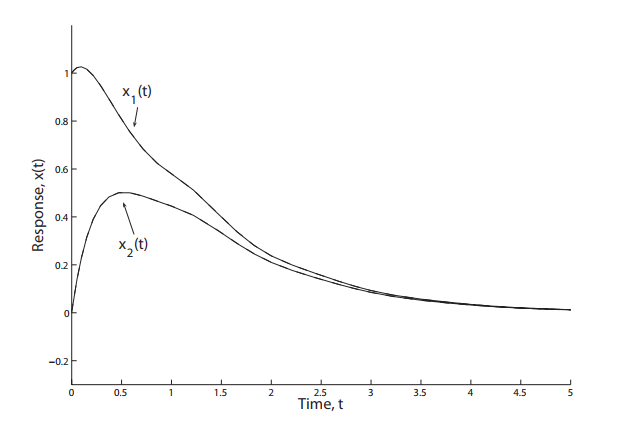
\includegraphics[width=0.5\linewidth]{hinh/hinh1a} &
		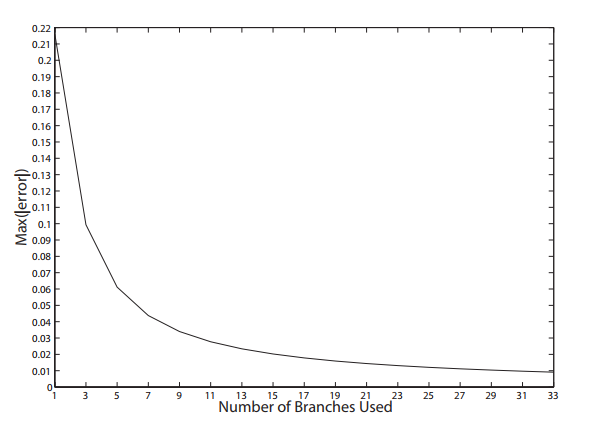
\includegraphics[width=0.5\linewidth]{hinh/hinh1b}\\
		(a) & (b)
	\end{tabular}
	\caption{Phản hồi trong Ví dụ \ref{vidu3} thu được bằng việc sử dụng $33$ nhánh đầu tiên của hàm Lambert (a) và sai số tuyệt đối của việc xấp xỉ phản hồi (b). Sai số sẽ tiếp tục giảm khi tiếp tục thêm những nhánh mới vào quá trình xấp xỉ phản hồi.}
	\label{n.hinh1}	
\end{figure}

Sử dụng tiêu chuẩn trong Mục \ref{sec2.3.1}, ta thấy hệ \eqref{t19} là điều khiển được theo điểm. Cho $B=[1\quad 0]^T$ chúng ta có thể tính toán ma trận điều khiển được Gramian $\mathcal{C}(0,t_1)$ trong \eqref{t8}. 
Do đó để hệ \eqref{t19} là điều khiển được theo điểm thì $\mathcal{C}(0,t_1)$ phải khả nghịch, tức là 
%
\begin{equation}\label{t20}
\det|C(0,t_1)| \not= 0.
\end{equation} 

Trong Hình \ref{n.refhinh2} chúng ta đi tính toán số cho định thức của ma trận $\cC(0,t_1)$ khi số nhánh tăng lên. Khi nhiều nhánh hơn được sử dụng thì nghiệm xấp xỉ sẽ hội tụ (xem Hình \ref{n.hinh1}), và điều tương tự cũng đúng với hàm hạch $\mathbf{K}(\xi,t)$ trong \eqref{t7} và ma trận điều khiển Gramian $\cC(0,t_1)$ trong \eqref{t8}. Hình \ref{n.refhinh2} cho thấy định thức hội tụ đến một giá trị khác không, có nghĩa là hệ thống là điều khiển được theo điểm.
%    
\begin{figure}[t]
	\centering
	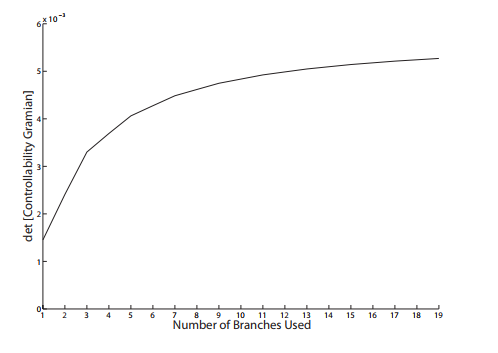
\includegraphics[width=0.7\linewidth]{hinh/hinh2n}
	\caption{Xấp xỉ định thức của ma trận điều khiển Gramian. Khi nhiều nhánh hơn được sử dụng, các định thức có xu hướng hội tụ về một giới hạn khác không.}
	\label{n.refhinh2}
\end{figure}   
%

Mặc dù một hệ thống thỏa mãn các điều kiện đại số được phát biểu trong các nghiên cứu trước đây như \cite{LeeOl81}, \cite{Mal87}, trong trường hợp định thức của ma trận quan sát Gramian trong \eqref{t16} nhỏ hơn một giá trị cụ thể nào đó thì việc thiết kế một bộ quan sát như trong \cite{LeeOl81}, \cite{Mal87}
có thể không hiệu quả. Lí do là vì hàm phạt (gain) thu được khi quan sát có thể trở nên cao một cách phi thực tế. Định thức của ma trận quan sát Gramian của hệ \eqref{t19} trong hai trường hợp $C=[0\quad 1]$ và $C=[1\quad 0]$ được so sánh trong Hình \ref{n.refhinh3} với $t_1=4$. Khi có thêm nhiều nhánh mới được sử dụng, giá trị của định thức trong trường hợp $C=[1\quad 0]$ có xu hướng hội tụ đến giá trị cao hơn so với trường hợp $C=[0 \quad 1]$.

\begin{figure}[t]
	\centering
	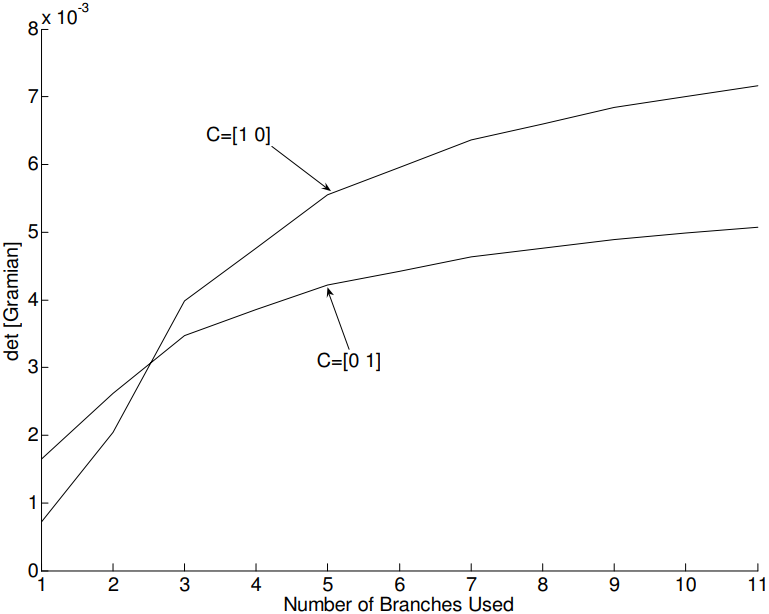
\includegraphics[width=0.6\linewidth]{hinh/hinh3n}
	\caption{Định thức của ma trận quan sát Gramian khi $C=[0\quad 1]$ và $C=[1\quad 0]$.}
	\label{n.refhinh3}
\end{figure}        
%  

Từ các kết quả trong Hình \ref{n.refhinh2} và \ref{n.refhinh3}, mặc dù một nghiên cứu chính thức về sai số chặt cụt là cần thiết, ta cũng có thể quan sát được sự hội tụ của Gramian khi số nhánh của hàm Lambert được sử dụng tăng thêm. Bởi vì ma trận điều khiển Gramian trong phương trình \eqref{t8} và ma trận quan sát Gramian trong phương trình \eqref{t16} là tích phân của tích của hàm hạch và ma trận hằng ($B$ và $C$) trên một khoảng hữu hạn, do đó sự hội tụ của các Gramians cũng được đảm bảo.
\end{vd}

Các kết quả được trình bày trong mục này là phù hợp với những kết quả thu được bằng các phương pháp đại số hiện có. Tuy nhiên, bằng cách sử dụng phương pháp Gramian được phát triển trong phần này, ta có thêm được một số thông tin. Ví dụ như ma trận điều khiển và ma trận quan sát Gramian cho biết làm thế nào để điều khiển và quan sát các trạng thái tương ứng \cite{Hol96}, trong khi các điều kiện đại số cho tính điều khiển được/tính quan sát được chỉ cho biết hệ là điều khiển/quan sát hoặc không. 
%
Do đó, thông qua những thay đổi đối với các ma trận Gramian, chúng ta cũng có thể xác định được sự thay đổi trong một số tham số của hệ hoặc độ trễ thời gian $h$ sẽ ảnh hưởng thế nào đến tính điều khiển được và tính quan sát được của hệ.

Trong lý thuyết điều khiển của các hệ thống tuyến tính không trễ, có một bài toán quan trọng có tên là \emph{bài toán nhận thức cân bằng (balanced realization)}. 
Bài toán nhận thức cân bằng được nghiên cứu bởi vì nhiều tính chất tốt của hệ biến đổi và mối liên hệ chặt chẽ của nó với việc điều khiển đa biến bền vững, xem \cite{Ver83}. Trong bài toán này, chúng ta cần đi tìm một phép đổi tọa độ có dạng $\hat{x}=\mathbf{Tx}(t)$ sao cho đối với hệ mới, các ma trận điều khiển/quan sát  Gramian bằng nhau và có dạng chéo. Sử dụng các ma trận Gramian trong Mục \ref{sec2.3}, ta có thể nghiên cứu bài toán tương tự cho các hệ điều khiển có trễ. Tính đến nay (2020), đây vẫn đang là một hướng nghiên cứu rất mới.

Đặt $\hat{x}=\mathbf{T} x(t)$. Khi đó tác động tương ứng trên các Gramians là
%
\begin{equation}\label{t21}
\hat{\mathcal{C}}(0,t_1)=\mathbf{T}\mathcal{C}(0,t_1)\mathbf{T}^T, \quad\hat{\mathcal{O}}(0,t_1)=\mathbf{T}^{-T}\mathcal{O}(0,t_1)\mathbf{T}^{-1}.
\end{equation}
%
Bằng việc chọn $\mathbf{T}$ thích hợp ta cần có $\hat{\mathcal{C}}(0,t_1) = \hat{\mathcal{O}}(0,t_1)$ và có dạng chéo. Trong Ví dụ \ref{vidu3}, với $B=[1\quad 0]^T$ và $C=[1\quad 0]$, $t_1=4$, sử dụng 11 nhánh của hàm ma trận Lambert W ta tìm được $\mathcal{C}(0, t_1)$, $\mathcal{O}(0,t_1 )$ lần lượt là
\begin{equation}\label{t22}
\mathcal{C}(0, t_1)=\begin{bmatrix}
0.2992 & 0.1079\\
0.1079 & 0.0554
\end{bmatrix}, \quad 
\mathcal{O}(0, t_1)=\begin{bmatrix}
0.2992 & -0.1484\\
-0.1484 & 0.0975
\end{bmatrix}. 
\end{equation}      
%
Trong trường hợp này, sử dụng ma trận
\begin{equation}\label{t23}
\mathbf{T} = \begin{bmatrix}
-0.3929 & 1.1910\\
1.0880 & -0.5054
\end{bmatrix},
\end{equation}
ta có
\begin{equation}\label{t24}
\hat{\mathcal{C}}(0,t_1)=\hat{\mathcal{O}}(0,t_1)=\begin{bmatrix}
0.0238 & 0.0000\\
0.0000 & 0.2497
\end{bmatrix}.
\end{equation}
%
Trong tương lai, chúng ta cần tiếp tục nghiên cứu để (1) thiết lập các điều kiện cho sự tồn tại của phép biến đổi $\mathbf{T}$ để đạt được sự nhận thức cân bằng cho DDE, và (2) phân tích sự hội tụ của $T$ khi số lượng nhánh được sử dụng tăng lên.  

%
\begin{table}[!]
	\scriptsize
	\begin{tabular}{lp{9cm}}
		\hline 
		ODEs & DDEs \\ 
		\hline 
		Tính điều khiển được & Tính điều khiển được theo điểm \\ 
		
		$\mathcal{C}(0,t_1)\equiv\int^{t_1}_0e^{A(t_1-\xi)}\mathbf{BB}^T\left(e^{A(t_1-\xi)}\right)^Td\xi$ & $\mathcal{C}(0,t_1)\equiv\int^{t_1}_0\sum\limits^\infty_{k=-\infty}e^{\mathbf{S}_k(t_1-\xi)}C^N_k\mathbf{BB}^T\left(\sum\limits^\infty_{k=-\infty}e^{\mathbf{S}_k(t_1-\xi)}C^N_k\right)^Td\xi$ \\ 
		
		$(s\mathbf{I}-A)^{-1}B$ & $(s\mathbf{I}-A-A_de^{-sh})^{-1}B$ \\ 
		
		$e^{A(t-0)}B$ & $\sum\limits^\infty_{k=-\infty}e^{\mathbf{S}_k(t-0)}C^N_kB$ \\ 
		\hline 
		Tính quan sát được & Tính quan sát được theo điểm \\ 
		
		$\mathcal{O}(0,t_1)\equiv\int^{t_1}_0\left(e^{A(\xi -0)}\right)^TC^TCe^{A(\xi-0)}d\xi$ & $\mathcal{O}(0,t_1)\equiv\int^{t_1}_0\left(\sum\limits^\infty_{k=-\infty}e^{\mathbf{S}_k(\xi -0)}C^N_k\right)^TC^TC\sum\limits^\infty_{k=-\infty}e^{\mathbf{S}_k(\xi -0)}C^N_kd\xi$ \\ 
		
		$C(s\mathbf{I}-A)^{-1}$ & $C(s\mathbf{I}-A-A_de^{-sh})^{-1}$ \\ 
		
		$Ce^{A(t-0)}$ & $C\sum\limits^\infty_{k=-\infty}e^{\mathbf{S}_k(t-0)}C^N_k$ \\ 
		\hline 
	\end{tabular}
	\caption{So sánh các tiêu chuẩn về tính điều khiển được và tính quan sát được đối với các hệ thống ODEs và DDEs}
\end{table}  
%   

\begin{vd} (Phân tích tính quan sát được và tính điều khiển được sử dụng gói công cụ LambertWDDE)
Xét phương trình \eqref{13}, với $A,A_d$ và $h$  được xác định trong Ví dụ 3 và
	\begin{equation*}
	B=\begin{bmatrix}
	1\\
	0
	\end{bmatrix}
	\hspace{1cm}
	\text{và}
	\hspace{1cm}
	C=\begin{bmatrix}
	0&1
	\end{bmatrix}
	\end{equation*}
\end{vd}
%
Hàm \textit{pwcontr\_test} có thể được sử dụng để kiểm tra tính điều khiển được của hệ. Nó kiểm tra hạng của ma trận $(s\mathbf{I}-A-A_de^{-sh})^{-1}B$ để xác định xem hệ có thể điều khiển được theo từng điểm hay không. Tính quan sát được theo từng điểm có thể được thiết lập bằng cách sử dụng hàm \textit{pwobs\_test}. Hơn nữa, tính điều khiển được và quan sát được trong một khoảng thời gian cụ thể có thể được tính toán xấp xỉ, sử dụng hàm \textit{ contr\_gramian\_dde} và \textit{obs\_gramian\_dde} tương ứng.


\section{Phân tích và điều khiển các hệ có trễ sử dụng gói công cụ LambertWDDE}
Trong mục này chúng ta sẽ sử dụng gói công cụ LambertWDDE để phân tích các tính chất điều khiển của các hệ điều khiển có trễ nảy sinh từ một số bài toán ứng dụng trong công nghiệp.

\subsection{Phân tích sự rung lắc của máy công cụ}

Sự rung lắc của máy công cụ, có thể được mô hình hóa như một hệ thống có trễ, là một trong những hạn chế chính làm hạn chế năng suất của quá trình tiện. Sự rung lắc này xảy ra không phải bởi vì tác động của ngoại lực, mà được gây ra bởi sự tương tác giữa cấu trúc máy và quá trình cắt. 

%Sự tương tác giữa cấu trúc phôi công cụ và quá trình cắt có thể được mô tả như một hệ kín (xem Hình \ref{fig:machinetoolchatter}). 

Nếu hệ thống này không ổn định (tức là hệ phương trình có trễ mô tả cho quá trình đó có ít nhất một giá trị riêng với phần thực dương), khi đó sự rung lắc có thể sẽ gây ra sự cố và dẫn đến bề mặt tiện bị kém phẩm chất đi, sự không chính xác về chiều trong bộ phận gia công và làm hư hỏng một phần hay hỏng hoàn toàn máy công cụ.

Tiếp theo các lý thuyết  về sự rung lắc cổ điển được giới thiệu bởi Tobias (1965) và Tlusty (2000) vào những năm 1960, nhiều mô hình khác nhau đã được phát triển để dự đoán sự khởi đầu của quá trình rung lắc. Tobias (1965) đã phát triển một phương pháp hình học và một phương pháp đại số để xác định sự khởi đầu của tính không ổn định cho một hệ thống có nhiều bậc tự do (DOF). Merritt (1965) đã trình bày một lý thuyết để tính toán ranh giới ổn định bằng cách vẽ các nghiệm điều hòa của phương trình đặc trưng của hệ thống, và cũng đề xuất một đường biên tiệm cận đơn giản để đảm bảo cho việc  không xảy ra dao động ở mọi tốc độ quay của trục chính. Optiz và Bernardi (1970) đã phát triển một biểu diễn vòng kín chung cho hai quá trình tiện và phay. 

Động lực học cấu trúc của máy được biểu thị theo các ma trận chuyển, trong khi quá trình cắt bị giới hạn bởi hai giả định: (1) hướng của lực cắt được cố định trong suốt quá trình cắt, và (2) các ảnh hưởng của tốc độ cung cấp vật liệu (feeding speed) và tốc độ cắt (cutting speed) bị bỏ qua . Những giả định này sau đó đã được bỏ qua bởi Minis (1990), người đã mô tả sự ổn định của hệ thống theo phương trình đặc trưng và sau đó áp dụng tiêu chuẩn ổn định Nyquist để xác định độ ổn định của hệ thống.  Ngoài ra, các tiêu chuẩn ổn định cho các hệ thống thời gian đã được phân tích bởi (Chen et al., 1997), Stepan (1989), Kuang (1993), và Stepan và Moon (1997), và sử dụng Định lý mạch rẽ nhánh Hopf (Nayfeh et al., 1997; Kalmar-Nagy et al. , 2001; Fofana, 2003). 

Gần đây, Olgac và Sipahi đã phát triển một cách tiếp cận mới dựa trên việc xử lý cụm nghiệm đặc trưng, kiểm tra một cụm nghiệm vô hạn tại một thời điểm để ổn định hệ thống trì hoãn để cho phép xác định vùng ổn định hoàn toàn của độ trễ (Sipahi và Olgac, 2003b), (Olgac và Sipahi, 2005). 
Trong mục này, cách tiếp cận dựa trên hàm ma trận Lambert W cho bài toán ổn định rung lắc được trình bày.  Sử dụng phương pháp này, người ta có thể có được phạm vi tốc độ quay trục chính mà không gây ra rung lắc. 

\begin{figure}[h!]
	\centering
	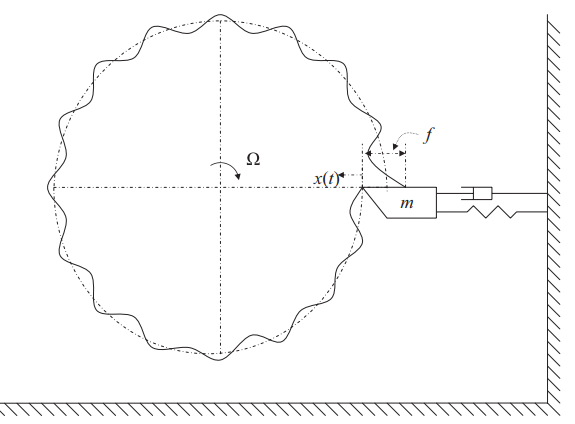
\includegraphics[width=0.7\linewidth]{hinh/machine_tool_chatter}
	\caption{Mô hình máy cắt vuông góc một bậc tự do, \cite[Chương 3]{Yi10}}
	\label{fig:machinetoolchatter}
\end{figure}

Trong quá trình tiện, một phôi hình trụ quay với vận tốc góc không đổi, và công cụ tạo ra một bề mặt khi vật liệu được tiện bỏ. Bất kỳ rung động nào của dụng cụ đều được thể hiện trên bề mặt này, điều đó có nghĩa là lực cắt phụ thuộc vào vị trí của dao tiện đối với vòng tiện hiện tại cũng như vòng tiện trước đó. Do đó, các phương trình vi phân có trễ đã được sử dụng rộng rãi làm mô hình cho máy công cụ. Mô hình cắt vuông góc một bậc tự do được mô tả trong Hình \ref{fig:machinetoolchatter}, có thể được biểu thị như (Kalmar-Nagy et al., 2001)
%
\begin{align}\label{turning process}
&\ddot{x}(t) + 2 \xi \omega_n  \dot{x}(t) + \left( \omega_n^2 + \dfrac{k_c}{m}\right) x(t) - \dfrac{k_c}{m} x(t-\tau ) \notag \\
& = \dfrac{k_c}{8 f_0 m} \left( (x(t) - x(t-\tau) )^2 - \dfrac{5}{12 f_0} (x(t) - x(t-\tau) )^3 \right),  
\end{align}
%
trong đó $x (t)$ là tọa độ tổng quát của vị trí cạnh dao, độ trễ $\tau = \dfrac{2\pi}{\omega_n}$ là khoảng thời gian cho một vòng quay, với $\omega_n$ là vận tốc góc của phôi quay. Hệ số $k_c$ là hệ số cắt xuất phát từ thực nghiệm của các tham số như chiều rộng chip, độ dày chip $f$ ($f_0$  là ở trạng thái ổn định) và tốc độ cắt. Tần số góc tự nhiên của hệ dao động tự do không chịu đẩy là $\omega_n$ và $\xi$ là hệ số giảm chấn tương đối. Lưu ý rằng giá trị $0$ của tọa độ tổng quát $x(t)$ của vị trí cạnh dao được chọn sao cho thành phần $x$ của lực cắt cân bằng với độ cứng khi độ dày chip $f$ có giá trị $f_0$ ( Kalmar-Nagy et al., 2001).

\noindent Đặt $x_1(t) = x(t)$ và $x_2(t) = \dot{x}(t)$, ta có thể chuyển hệ bậc hai \eqref{turning process} về hệ bậc nhất 
%
\begin{align}\label{turning proceess 2}
\dot{x}_1(t) &= x_2(t), \notag \\
\dot{x}_2(t) &= 2 \xi \omega_n {x}_2(t) + \left( \omega_n^2 + \dfrac{k_c}{m}\right) x_1(t) - \dfrac{k_c}{m} x_1(t-\tau ) \notag \\
& \quad + \dfrac{k_c}{8 f_0 m} \left( (x_1(t) - x_1(t-\tau) )^2 - \dfrac{5}{12 f_0} (x_1(t) - x_1(t-\tau) )^3 \right),  
\end{align}
%
Giả sử rằng không có dao động nào trong vòng tiện trước, tức là $x_1(t-\tau) = 0$, thì ta có thể tìm được điểm cân bằng $x_1(t)=x_2(t) = 0$, 
có nghĩa là tại điểm cân bằng này, cạnh dao nằm tại vị trí như được xác định trước đó.
Tuyến tính hóa hệ tại điểm cân bằng chúng ta thu được
%
\begin{equation}\label{eq3}
\m{\dot{x}_1(t) \\ \dot{x}_2(t)} = \m{0 & 1 \\ -\left( \omega_n^2 + \dfrac{k_c}{m}\right) & - 2 \xi \omega_n } \m{{x}_1(t) \\ {x}_2(t)} 
+ \m{0 & 0 \\ \dfrac{k_c}{m} & 0 } \m{{x}_1(t-\tau) \\ {x}_2(t-\tau)} \ .
\end{equation}
%
Với $k_m := m \omega_n^2$ được gọi là \emph{độ cứng cấu trúc} (N/m), ta có thể viết lại hệ \eqref{eq3} như sau
%
\begin{equation}\label{eq4}
\m{\dot{x}_1(t) \\ \dot{x}_2(t)} = \m{0 & 1 \\ - \omega_n^2 \left( 1 + \dfrac{k_c}{k_m}\right) & - 2 \xi \omega_n } \m{{x}_1(t) \\ {x}_2(t)} 
+ \m{0 & 0 \\ \dfrac{k_c}{k_m}\omega_n^2 & 0 } \m{{x}_1(t-\tau) \\ {x}_2(t-\tau)} \ .
\end{equation}
%
Chú ý rằng sự rung lắc sẽ xảy ra nếu như hệ \eqref{eq4} không ổn định. 

Cách tiếp cận dựa trên hàm Lambert W cho thấy điều kiện ổn định cho hệ \eqref{t1} phụ thuộc vào các giá trị riêng của ma trận $S_k$. Khi đó ta có hệ \eqref{t1} là ổn định không điều kiện khi và chỉ khi tất cả các giá trị riêng của $S_k$ có phần thực âm. 

Ví dụ ta xét trường hợp tốc độ quay trục chính $1/T$ = 50, $\omega_n = 150$ ($Hz^2$) và $\xi = 0.05$, tỉ số $\dfrac{k_c}{k_m} = 0.25$.
Khi đó các ma trận $S_k$ và các giá trị riêng tương ứng thu được qua tính toán là như trong Bảng \ref{bang 3}.

\begin{table}[!h]
\centering
\begin{tabular}{lcc}
\hline \\[-.35cm]	
Chỉ số nhánh & $S_{k_1,k_2}$ & Giá trị riêng của $S_{k_1,k_2}$ \\ \hline \\[-.35cm]
$k_1 = k_2 = 0$		   & $\m{0 & 1 \\ -33083 & -0.24}$ & $-0.12 \pm 181.88 i$ \\ \hline \\[-.35cm]
$k_1 = -1$, $k_2 = 0$  & $\m{0 & 1 \\ -77988 + 32093i & -177 - 247i }$ &  
$\pma{- 0.12 + 181.88 i \\ -176.73 - 428.66i}$ \\ 
$k_1 = 0$, $k_2 = -1$	& $\m{0 & 1 \\ -11 - 1663i & -92 - 182i}$  &  $\pma{ -91.61 \\ - 0.12-181.88i}$ \\ \hline \\[-.35cm]
$k_1 = 1$, $k_2 = 0$   & $\m{0 & 1 \\ -77988 - 32093i & -177 + 247i}$ &  
$\pma{- 0.12 - 181.88 i \\ -176.73 + 428.66i}$ \\ 
$k_1 = 0$, $k_2 = 1$	& $\m{0 & 1 \\ -11 + 1663i & -92 + 182i}$  &  $\pma{ -91.61 \\ - 0.12-181.88i}$ \\ \hline \\[-.35cm]
$\vdots$ & $\vdots$ & $\vdots$ \\ \hline
\end{tabular} 
\caption{Tính toán các ma trận $S_k$ và các giá trị riêng trội}
\label{bang 3}
\end{table}

Thêm vào đó, các giá trị riêng của ma trận $S_{0,0}$ là gần trục ảo nhất và phần thực của chúng là âm. Hơn nữa, sử dụng các nhánh bổ sung để tính toán giá trị riêng luôn đem lại các giá trị riêng mà phần thực của nó nằm ở bên trái trong mặt phẳng phức (xem Hình \ref{spectrumchatter-2}). 
Điều này hoàn toàn phù hợp với Phỏng đoán \ref{conj} và ta có thể dự đoán rằng hệ \eqref{eq4} với bộ tham số đang xét là ổn định không điều kiện.\

\begin{figure}[h!]
	\centering
	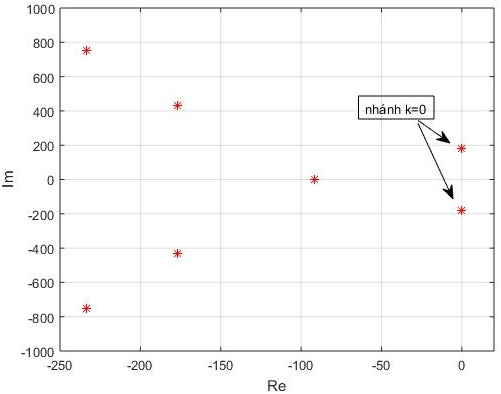
\includegraphics[width=0.7\linewidth]{hinh/spectrum_chatter-2}
	\caption{Giá trị riêng của hệ \eqref{eq4} trong mặt phẳng phức. Các giá trị riêng thu được bằng cách sử dụng nhánh chính (k = 0) là trội và sẽ quyết định tính ổn định của hệ.}
	\label{spectrumchatter-2}
\end{figure}

Chú ý rằng thực tế thông qua việc tính toán các giá trị riêng trội, sử dụng công cụ tính toán phổ trong \cite{Eng01}, ta biết rằng hệ \eqref{eq4} với bộ tham số đang xét là ổn định không điều kiện. \ 
Thêm vào đó, bằng việc quan sát các giá trị riêng của $S_{0,0}$ tương ứng với nhánh chính, người ta có thể tìm điểm tới hạn mà vượt qua ngưỡng đó thì sự rung lắc của máy tiện sẽ xảy ra. Ví dụ, khi tốc độ quay trục chính $1/T$ = 50, $\omega_n = 150$ ($Hz^2$) và $\xi = 0.05$, tỉ số $\dfrac{k_c}{k_m} = 0.2527$. Giá trị này vừa đúng bằng kết quả thu được bằng phương pháp Lyapunov (\cite{Mal87}), tiêu chuẩn Nyquist và phương pháp tính toán trong \cite{Che98}. Các ngưỡng ổn định theo phương pháp này được mô tả trong Hình \ref{fig:stability-lobes}, \cite[Chương 3]{Yi10}.

\begin{figure}[h!]
	\centering
	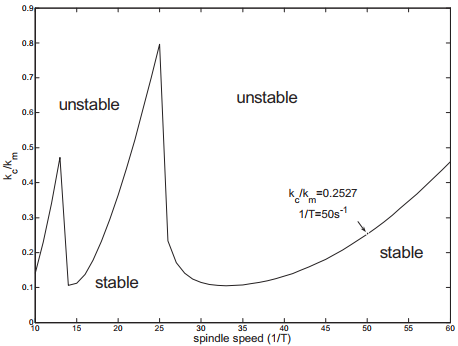
\includegraphics[width=0.8\linewidth]{hinh/stability-lobes}
	\caption{Các ngưỡng ổn định trong bài toán rung lắc của máy tiện}
	\label{fig:stability-lobes}
\end{figure}

\subsection{Điều khiển động cơ Diesel}

%Trong phần này, việc điều khiển động cơ diesel được xem là minh họa cho những lợi thế và tiềm năng của phương pháp được đề xuất trong Phần 7.3. Cụ thể, bộ điều khiển phản hồi và người quan sát được thiết kế thông qua việc gán giá trị riêng bằng cách sử dụng phương pháp dựa trên chức năng Lambert W. 

Một động cơ diesel có van tuần hoàn khí thải (EGR) và máy nén turbo với tuabin hình học biến thiên (VGT) đã được mô hình hóa trong \cite{JanK00} (Hình \ref{fig:dieselenginecontrol}) 
sử dụng 3 biến trạng thái sau: $x(t) = \m{x_1 & x_2 & x_3}^T$, $x_1$ là áp suất đường ống nạp, $x_2$ là áp suất đường ống xả và $x_3$ là công suất máy nén. Mô hình bao gồm độ trễ do khí vận chuyển trong đường ống nạp vào ống xả ($h = 60$ ms khi tốc độ động cơ $N$ là 1500 vòng/phút). 

\begin{figure}[h!]
	\centering
	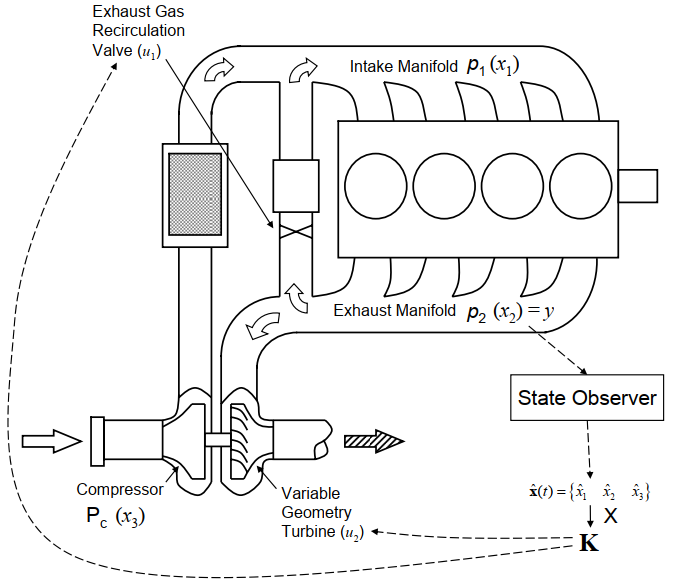
\includegraphics[width=0.7\linewidth]{hinh/diesel_engine_control}
	\caption{Điều khiển động cơ diesel bằng việc sử dụng đo đạc áp suất ống xả, tất cả các trạng thái đều sẽ được ước lượng thông qua bộ quan sát trạng thái và sau đó được sử dụng trong việc thiết kế điều khiển phản hồi (\cite{JanK09})}
	\label{fig:dieselenginecontrol}
\end{figure}

Do đó, một hệ có trễ được tuyến tính hóa dạng \eqref{t1} đã được giới thiệu trong \cite{JanK09} cho một điểm vận hành cụ thể (N = 1500 vòng/phút) có dạng
%
\begin{equation}\label{eq7}
\dot{x}(t) = \underbrace{\m{-27 & 3.6 & 6 \\ 9.6 & -12.5 & 0 \\ 0 & 9 & -5}}_{A} {x}(t) +   
\underbrace{\m{0 & 0 & 0 \\ 21 & 0 & 0 \\0 & 0 & 0 }}_{A_d} {x}(t-h) + 
\underbrace{\m{0.26 & 0 \\ -0.9 & -0.8 \\ 0 & 0.18}}_{B} {u}(t)  \ .
\end{equation}
%
Bên cạnh đó, bằng việc đặt một cảm biến quan sát tại ống xả, chúng ta sẽ đo áp suất xả. Do đó đầu ra của hệ điều khiển có trễ tương ứng với phương trình \eqref{eq7} là
%
\begin{equation}\label{eq5}
y(t) = \m{0 & 1 & 0} x(t) \ .
\end{equation}
%
\begin{figure}[h!]
	\centering
	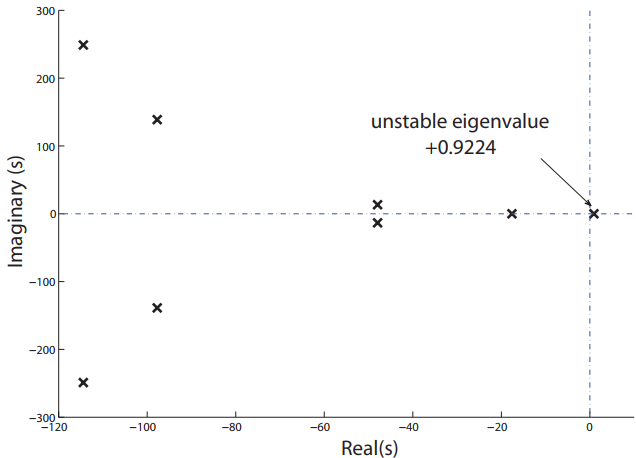
\includegraphics[width=0.7\linewidth]{hinh/spectrum_diesel}
	\caption{Phổ của hệ \eqref{eq7}, \cite{JanK09}.}
	\label{fig:spectrumdiesel}
\end{figure}
%
Chú ý rằng phổ của hệ \eqref{eq7} có chứa một giá trị riêng với phần thực dương (Hình \ref{fig:spectrumdiesel}), vì vậy hệ là không ổn định.
Bây giờ ta sẽ đi nghiên cứu tính điều khiển được và quan sát được của hệ thông qua các điều kiện phát biểu trong các Hệ quả \ref{coro 2}, \ref{coro 4} trong Mục \ref{sec2.3}. Ví dụ, để xét tính điều khiển được, ta có thể sử dụng gói công cụ Symbolic trong MATLAB để tính toán trực tiếp
%
\begin{equation*}
(s\mathbf{I}-A-A_d e^{-sh})^{-1}B 
= \m{ s + 27 &    -18/5 &    -6 \\ - 21 e^{-sh} - 48/5 & s + 25/2 &     0 \\ 0 & -9 & s + 5 }^{-1} \m{0.26 & 0 \\ -0.9 & -0.8 \\ 0 & 0.18}, 
\end{equation*}
%
và kiểm tra điều kiện hạng \eqref{t15}. Đó là cách làm được thực hiện trong hàm \linebreak \emph{pwcontr\_test} trong gói công cụ LambertWDDE.
Điều tương tự cũng được thực hiện với tính quan sát được, sử dụng 
hàm \emph{pwobs\_test} trong cùng gói công cụ. \ 
Khi đó, hệ điều khiển có trễ \eqref{eq7}-\eqref{eq5} vừa là điều khiển được theo điểm vừa là quan sát được theo điểm. Điều này phù hợp với những quan sát trong \cite{JanK09}.

